\chapter{FDTD Parameter Setup}
This is a chapter about the proper setup of all necessary FDTD parameter.

\section{Excitation signal setup}
This is a paragraph about the FDTD excitation signal setup

\subsection{Gaussian pulse}

\subsection{Sinousoidal signal}

\subsection{Other excitation signals}


\section{Boundary Conditions}
    Boundary conditions (BC) are necessary for solving the  Maxwell's equations by FDTD. Following are the theoretical general expressions for boundary conditions at an arbitrary interface of materials and/or surface currents:
    %%%%% BC EQ
	\begin{eqnarray}
	    \hat{n}\cdot(\vec{\mathbf{D}}_2-\vec{\mathbf{D}}_1) &=&\rho_s  \\
	    \hat{n}\cdot(\vec{\mathbf{B}}_2-\vec{\mathbf{B}}_1) &=&0  \\
	    \hat{n}\times(\vec{\mathbf{E}}_2-\vec{\mathbf{E}}_1) &=&-\vec{\mathbf{M}}_s \\
	    \hat{n}\times(\vec{\mathbf{H}}_2-\vec{\mathbf{H}}_1) &=&\vec{\mathbf{J}}_s
	    \label{eq:General boundary conditions}
	\end{eqnarray}
    %%%%% BC Diagrams
    Figure  \ref{fig:General BC diagrams} shows the above relations.
    \begin{figure}[ht]
      \centering
	  %\subfloat[CAPTION]{BILDERCODE}\qquad
	  \subfloat[$\vec{\mathbf{D}}$]{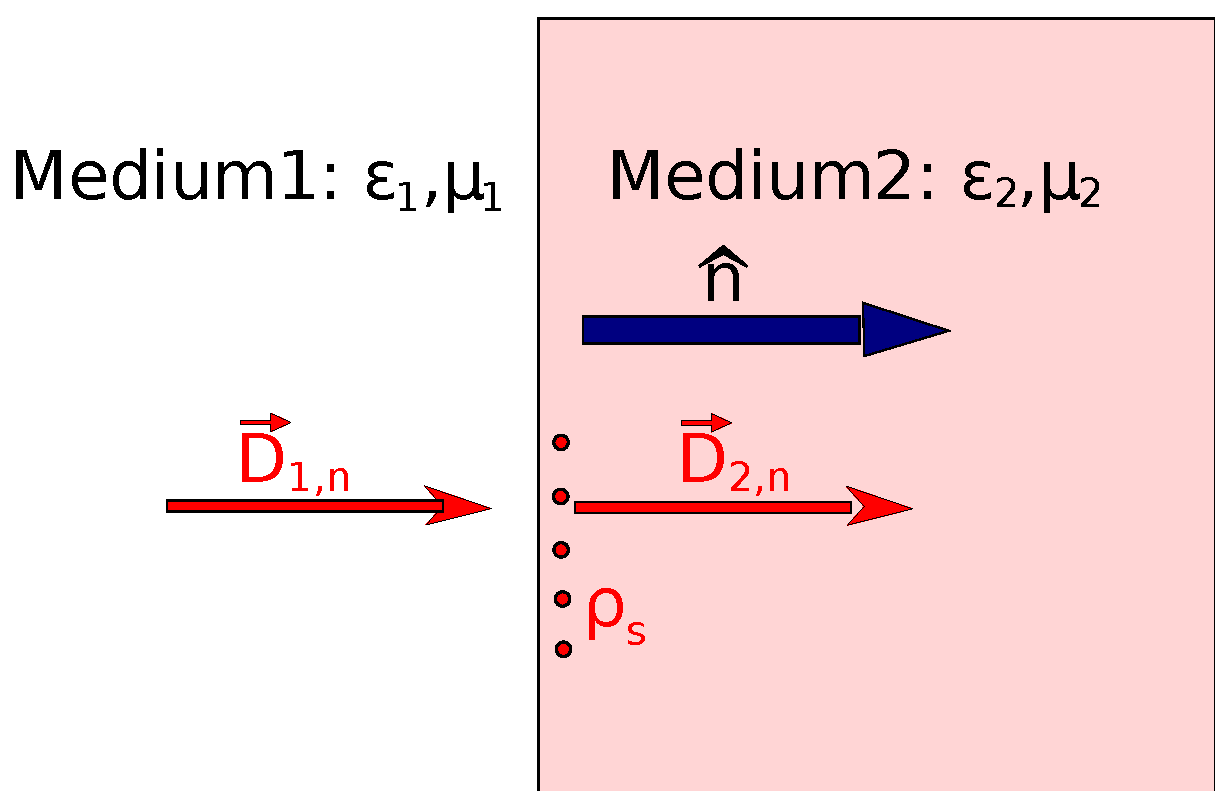
\includegraphics[width=0.4\textwidth]{svg/BC_general_Dn.eps}}\qquad
	  \subfloat[$\vec{\mathbf{B}}$]{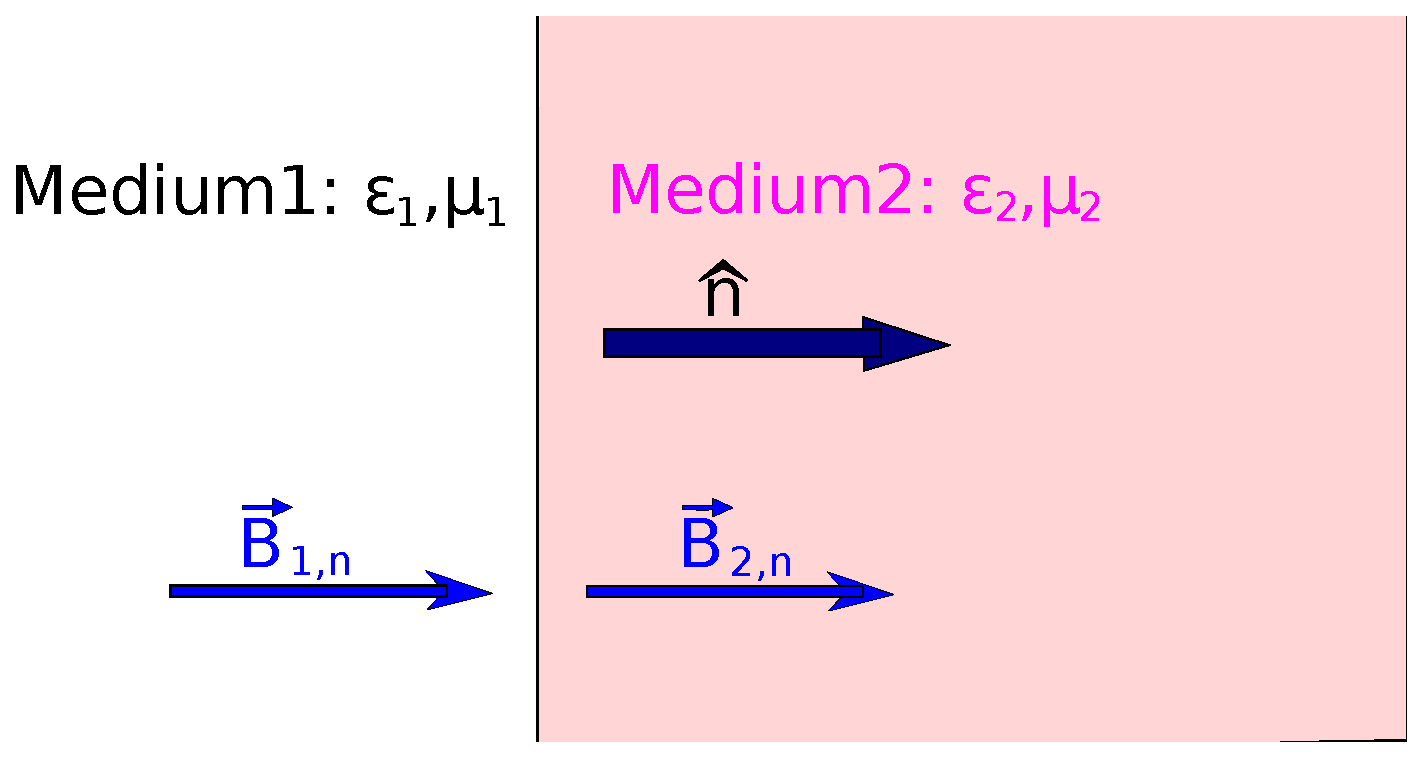
\includegraphics[width=0.4\textwidth]{svg/BC_general_Bn.eps}}\qquad 
	  \subfloat[$\vec{\mathbf{E}}$]{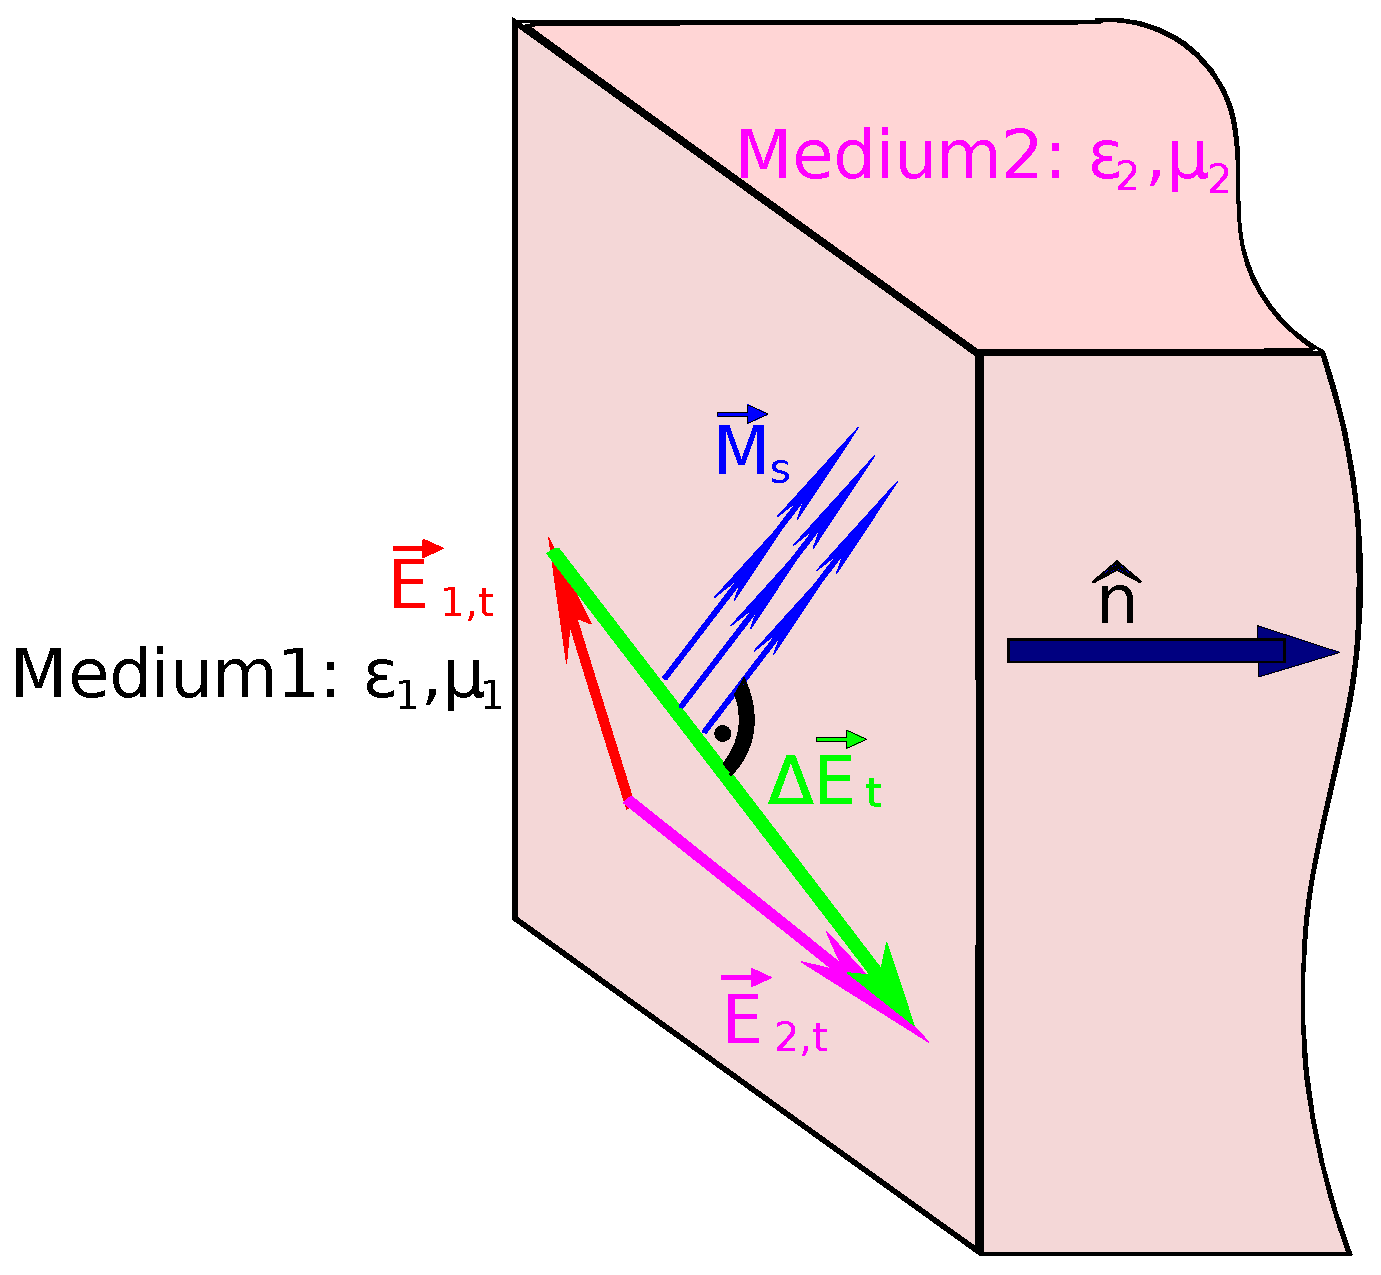
\includegraphics[width=0.4\textwidth]{svg/BC_general_Et.eps}}\qquad
	  \subfloat[$\vec{\mathbf{H}}$]{\includegraphics[width=0.4\textwidth]{svg/BC_general_Ht.eps}}\qquad 
	    \caption[General BC diagrams]{General boundary condition on an interface between 2 media for $\vec{\mathbf{D}}$, $\vec{\mathbf{B}}$, $\vec{\mathbf{E}}$ and $\vec{\mathbf{H}}$. n denotes normal components. t denotes tangential components. s denotes surface.}
	    \label{fig:General BC diagrams}
    \end{figure}

    In practice  under some special conditions or assumption, the boundary conditions(\ref{eq:General boundary conditions}) have  special forms, which are convenient for simulation. These BC are \textit{perfect electric conductor (\textbf{PEC}), perfect magnetic conductor (\textbf{PMC}), \textbf{MUR} absorbing boundary condition and perfectly matched layer (\textbf{PML}) absorbing boundary condition}.

     DEFINITION IN OPEN-EMS BY MATLAB [X X Y Y Z Z] [RHO RHO ALPHA ALPHA Z Z ]
     MESHES.......
     EXAMPLE
\subsection{Perfect electric conductor (PEC)}
This BC can be applied where the boundary are \textbf{good conductor(e.g., metals)}, because the metals can often be seen as lossless(conductivity $\sigma\rightarrow\infty$). So conditions for PEC are
%%%%% PEC CONDITIONS
\begin{itemize}
 \item \textbf{good conductor(e.g., metals)} or $\sigma\rightarrow\infty$
 \item $\vec{\mathbf{M}}_s=0$
\end{itemize}
The BC equations are
    %%%%% PEC BC EQ
	\begin{eqnarray}
	    \hat{n}\cdot\vec{\mathbf{D}}_1 &=&-\rho_s  \\
	    \hat{n}\cdot\vec{\mathbf{B}}_1 &=&0  \\
	    \hat{n}\times\vec{\mathbf{E}}_1 &=&0\\
	    \hat{n}\times\vec{\mathbf{H}}_1 &=&-\vec{\mathbf{J}}_s
	    \label{eq:PEC boundary conditions}
	\end{eqnarray}
    %%%%% PEC BC Diagrams
    Figure  \ref{fig:PEC BC diagrams} shows the above relations.
    \begin{figure}[ht]
      \centering
	  %\subfloat[CAPTION]{BILDERCODE}\qquad
	  \subfloat[$\vec{\mathbf{D}}$]{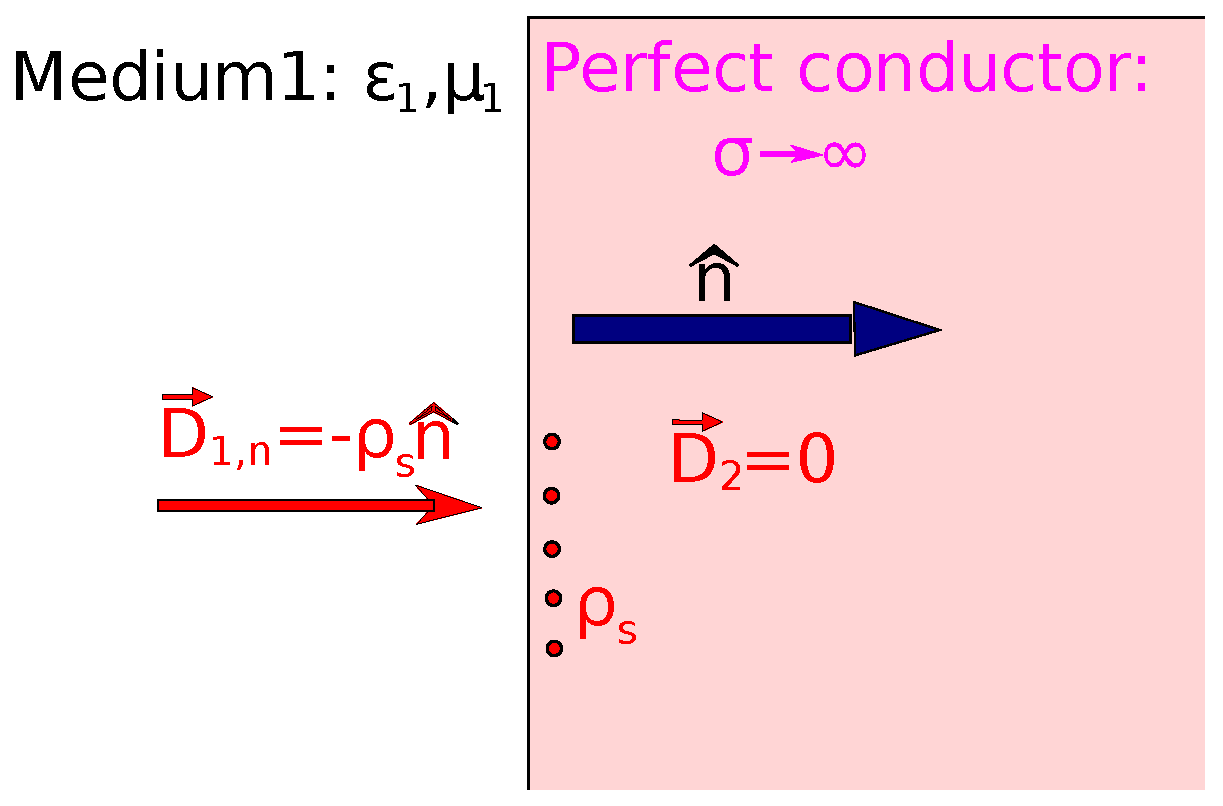
\includegraphics[width=0.4\textwidth]{svg/PEC_BC_general_Dn.eps}}\qquad
	  \subfloat[$\vec{\mathbf{B}}$]{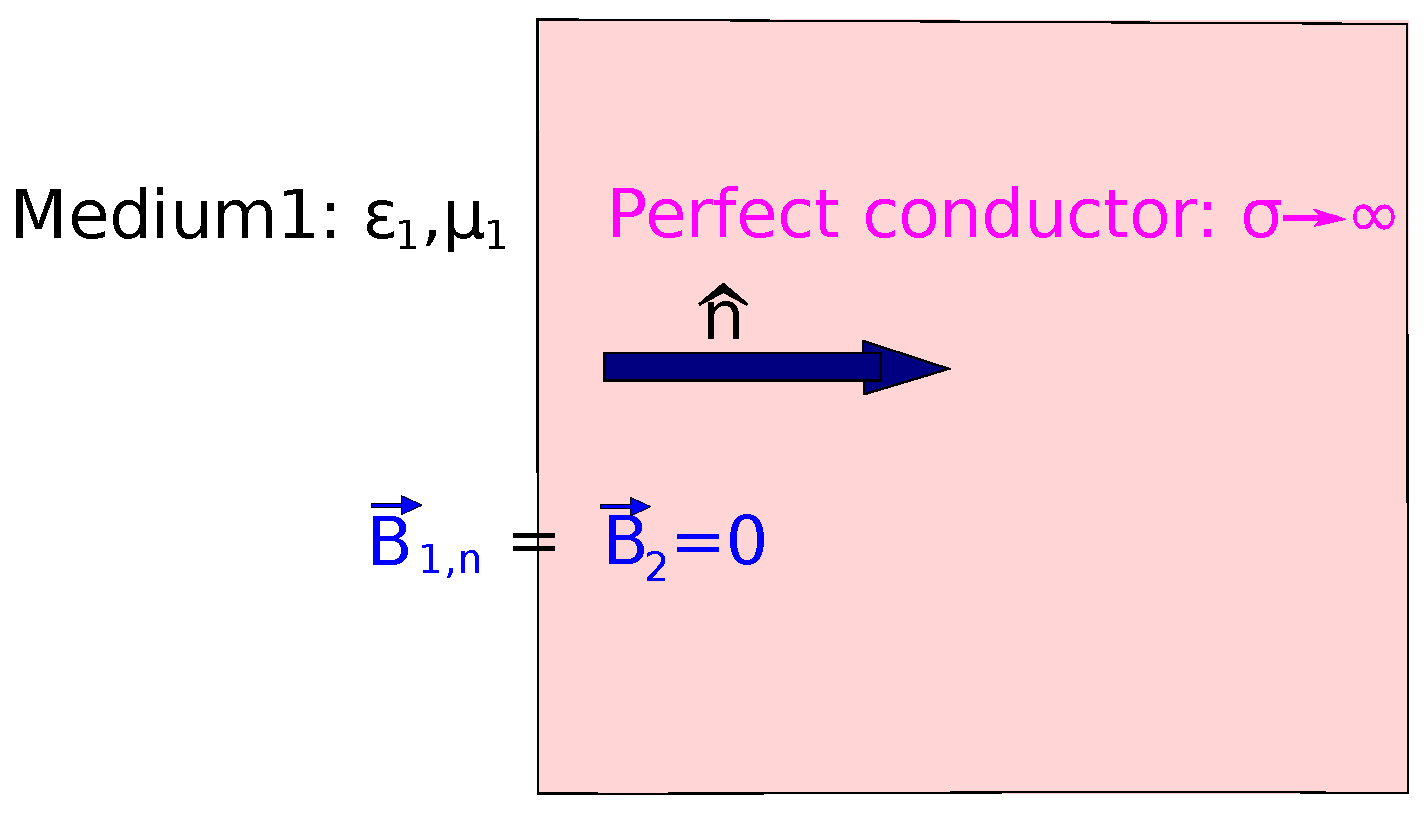
\includegraphics[width=0.4\textwidth]{svg/PEC_BC_general_Bn.eps}}\qquad 
	  \subfloat[$\vec{\mathbf{E}}$]{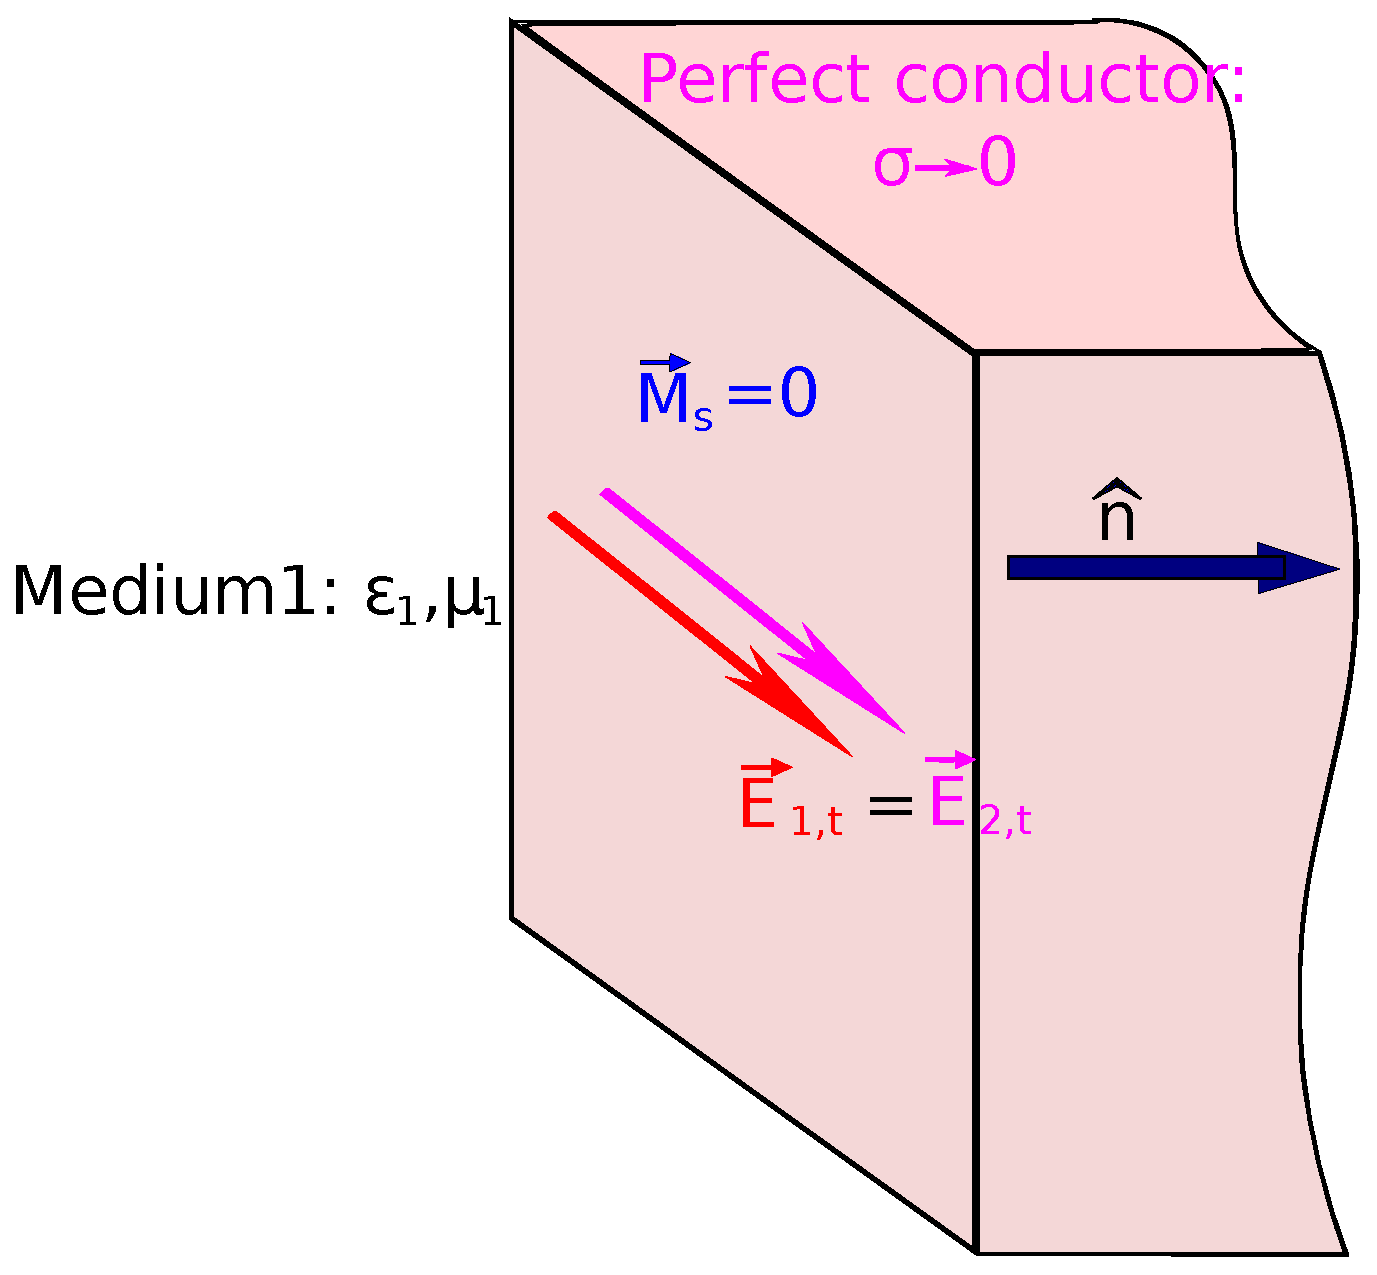
\includegraphics[width=0.4\textwidth]{svg/PEC_BC_general_Et.eps}}\qquad
	  \subfloat[$\vec{\mathbf{H}}$]{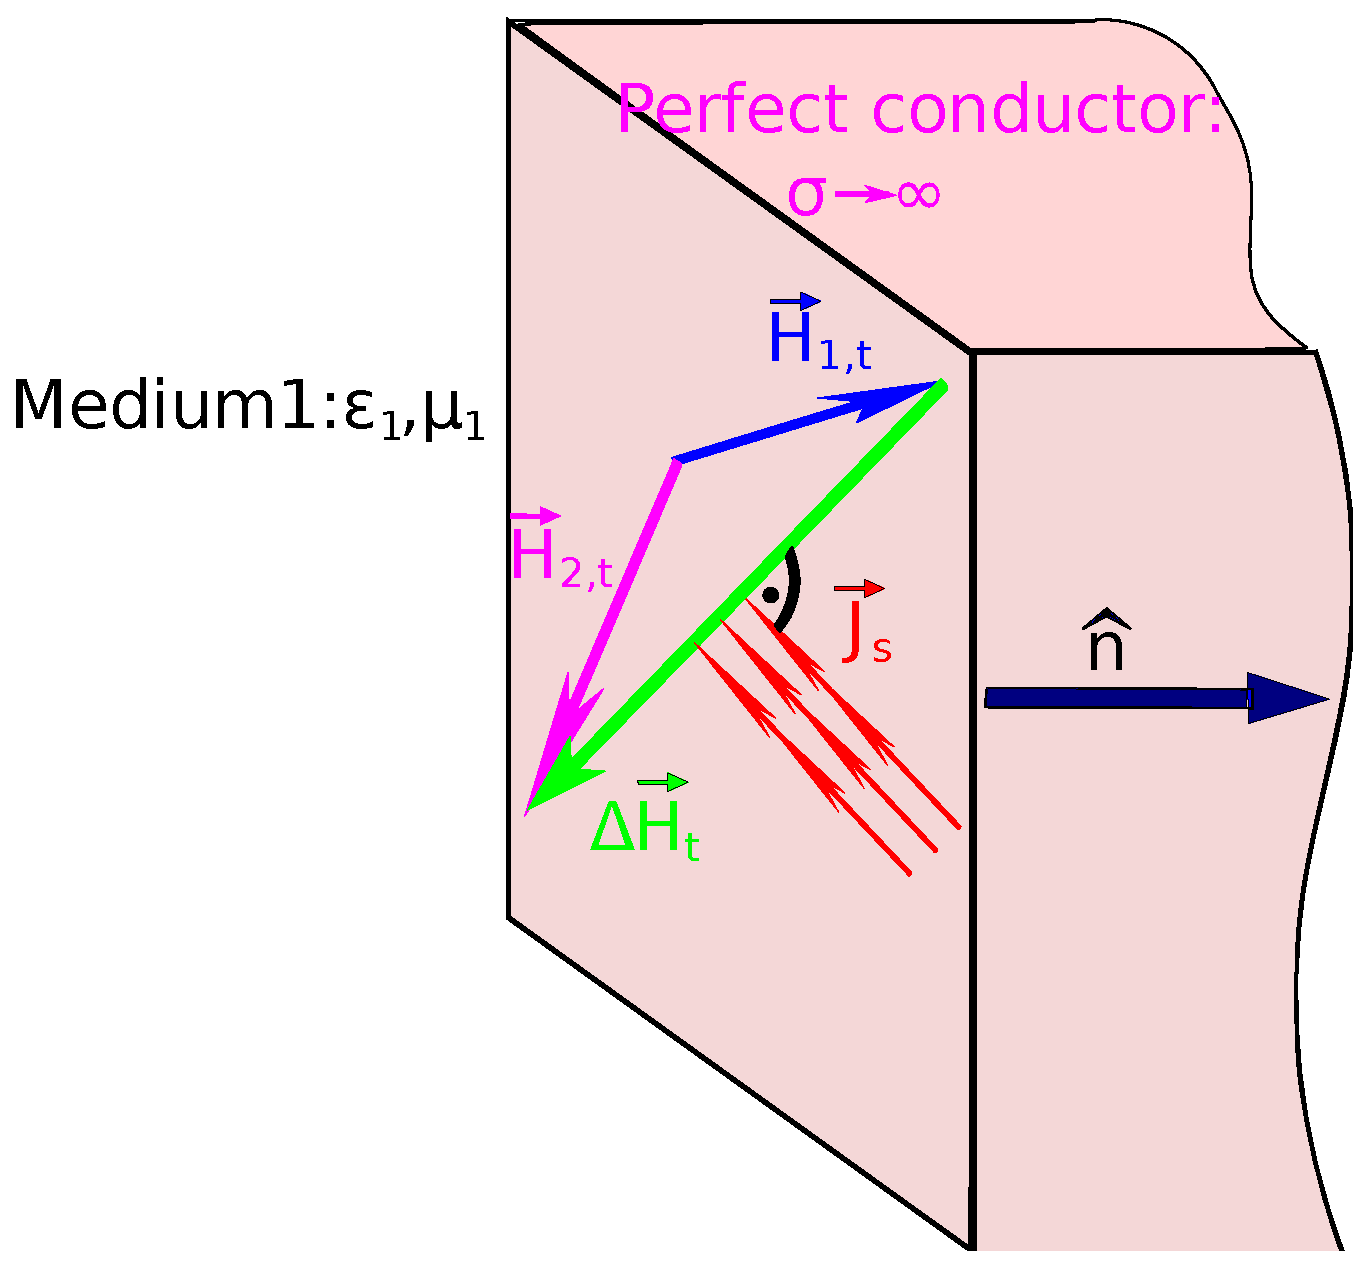
\includegraphics[width=0.4\textwidth]{svg/PEC_BC_general_Ht.eps}}\qquad 
	    \caption[PEC BC diagrams]{PEC boundary condition  for $\vec{\mathbf{D}}$, $\vec{\mathbf{B}}$, $\vec{\mathbf{E}}$ and $\vec{\mathbf{H}}$. n denotes normal components. t denotes tangential components. s denotes surface.}
	    \label{fig:PEC BC diagrams}
    \end{figure}

     DEFINETION IN OPEN-EMS BY MATLAB [X X Y Y Z Z] [RHO RHO ALPHA ALPHA Z Z ]
     MESHES.......
     EXAMPLE
\subsection{Perfect magnetic conductor (PMC)}

\subsection{MUR absorbing boundary condition}

\subsection{Perfectly matched layer (PML) absorbing boundary condition}
